

\subsection{Fysik teori}
Teoretisk udledning af formler til det skrå kast\\
Begyndelseshastigheden for et kast er givet ud fra vektoren $v_{0}$ og vinklen a, det betyder altså at hastighedsvektorens komposanter kan findes ved:\\

\begin{center}
\begin{math}
\centering
v_{x} = v_{0} \cdot cos(a) \quad \textrm{og} \quad v_{y} = v_{0} \cdot sin(a)
\end{math}
\end{center}

Samtidigt vides det at x- og y-slut kan skrives som to bevægelsesligninger:\\

\begin{center}
\begin{math}
\centering
y = -\dfrac{1}{2} \cdot g \cdot t^{2} + v_{y} \cdot t + y_{0}
\end{math}
\end{center}



Hvor dette er formlen for strækning inden for faget kinematik, omskrevet til at passe på y-aksen i det skrå kast. Her skiftes strækningen ud med y og accelerationen med g, da det er tyngdeaccelerationen som kastet arbejder imod:\\

\begin{center}
\begin{math}
\centering
s = -\dfrac{1}{2} \cdot g \cdot t^{2} + v_{0} \cdot t + s_{0} 
\end{math}
\end{center}

x er derved givet ved konstant hastighed, denne får altså ligningen:\\

\begin{center}
\begin{math}
\centering
x = v_{x} \cdot t
\end{math}
\end{center}

Hvor denne er omskrevet fra formlen for konstant hastighed:\\

\begin{center}
\begin{math}
\centering
v = \dfrac{\Delta s}{\Delta t}
\end{math}
\end{center}




Hvor der isoleres for strækningen:\\

\begin{center}
\begin{math}
v = \dfrac{\Delta s}{\Delta t} \longrightarrow \Delta s = v \cdot \delta t
\end{math}
\end{center}

Dette giver altså to ligninger for x- og y-slut nr komposanterne indsættes:\\

\begin{center}
\begin{math}
x_{slut} = v_{0} \cdot cos(a) \cdot t
\end{math}
\end{center}

og\\

\begin{center}
\begin{math}
y_{slut} = -\dfrac{1}{2} \cdot g \cdot t^{2} + v_{0} \cdot sin(a) \cdot t + y_{0}
\end{math}
\end{center}

\textbf{Bestemmelse af  $x_{slut}$}\\
I vores forsøg kender vi hverken tiden eller $x_{slut}$. Tiden kan dog bestemmes.\\

Det vides at $y_{slut}$ er lig $y_{0}$, da planet forsøget er udført på er ensartet, dette vil altså sige, at både $y_{o}$ og $y_{slut}$ er lig 0. Dette kan altså sættes ind i ligningen for $y_{slut}$ og der kan isoleres for t:\\

\begin{center}
\begin{math}
0 = -\dfrac{1}{2} \cdot g \cdot t^{2} + v_{y} \cdot t + y_{0} \longrightarrow t = \dfrac{v_{y} + \sqrt{2 \cdot g \cdot y_{0} + y^{2}_{y}}}{g}
\end{math}
\end{center}

Den tidligere bestemte y komposant kan indsættes så alle variabler kendes:\\

\begin{center}
\begin{math}
t = \dfrac{v_{0} \cdot sin(a) + \sqrt{2 \cdot g \cdot y_{0} + y^{2}_{y}}}{g}
\end{math}
\end{center}

\textbf{Opsat som vektorfunktion}\\
Vektorfunktioner er givet ud fra en ligning for bevægelsen på x-aksen og bevægelsen på y-aksen:

\begin{center}
\begin{math}
\overrightarrow{r}(t) = 
\begin{pmatrix}
x(t)\\
y(t)
\end{pmatrix}
\end{math}
\end{center}

Da bevægelser er beskrevet ved brug af vektorere opsættes skuddet som en vektorfunktion:

\begin{center}
\begin{math}
\overrightarrow{r}(t) = 
\begin{pmatrix}
v_{0} \cdot cos(a) \cdot t\\
- \dfrac{1}{2} \cdot g \cdot t^{2} + v_{0} \cdot sin(a) \cdot t + y_{0}
\end{pmatrix}
\end{math}
\end{center}

\subsection{Forsøg}
\subsubsection{Apparaturliste}
\begin{itemize}
\item 2x opsætnings stativer
\item 1x BT5 A5 Elektrisk Airsoft Gevær
\item 1x LiDAR af typen Leica “Disto D5”
\item 1x Tomstok
\end{itemize}

\subsubsection{Fremgangsmåde}

\begin{figure}[H]
\centering
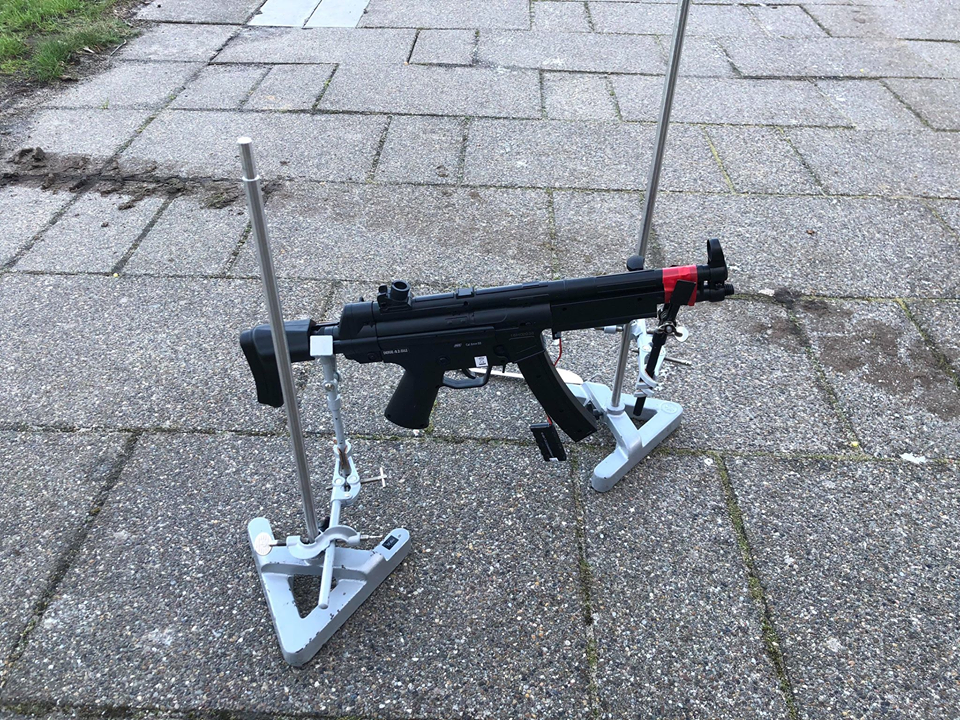
\includegraphics[scale=0.4]{Billeder/Opstilling.png}
\caption{Forsogsopstilling.}
\label{fig:Opstilling}
\end{figure}


\begin{enumerate}
\item Først opsættes det elektriske airsoft gevær på en sådan måde at vinklen er let at ændre, denne opsætning ses på figur \ref{fig:Opstilling}.

\item Der indstilles en vinkel. 
\begin{enumerate}
\item Højden mellem de to monteringspunkter og jorden måles.
\item Der måles en afstand mellem de to monteringspunkter, dette er en hypotenuse mellem de to monteringspunkter.
\item det lave monteringspunkt trækkes fra det høje, og nu er en modstående katete til den ønskede vinkel fundet.
\item Bestem brugt vinkel ud fra sinus beregning.
\end{enumerate}

\item Skud affyres.

\item Afstanden fra skuddets første kontaktpunkt med jorden hen til gevær-opstillingen ved hjælp af LiDAR.

\item Der tages tre målinger for hver vinkel.
\end{enumerate}











